\section{\green{Methods}}

I am following the assumption that we don't start from a blank slate but from some initial concepts, here operationalized as primitives, fundamental program components. These initial primitives comprise a minimal domain-specific language (DSL) and can be composed into more complex programs, which represent the causal structure generating the observations we perceive. As such, an agent learns its own DSL, which in terms of a language of thought is analogous to inferring a mental grammar and using it to learn new concepts.



\subsection{\green{Computational Model}}



\subsubsection{\green{DeepSynth Framework}}

Both in DreamCoder and DeepSynth, programs are represented as abstract syntax trees (ASTs). An AST is a tree representation of the syntactic structure of the program, with nodes representing operations or primitives and edges representing their compositional relationships. In order to avoid predicting variables, deBruijn indexing is used, which is a technique to represent bound variables in a way that avoids naming conflicts and simplifies variable substitution \cite{de_Bruijn_1972}. Named variables are replaced with numeric indices representing the number of enclosing $\lambda$ abstractions that bind the variable. See figure \ref{fig:AST} for a visualization of an AST using deBruijn indexing.

\begin{figure}[H]
    \centering
    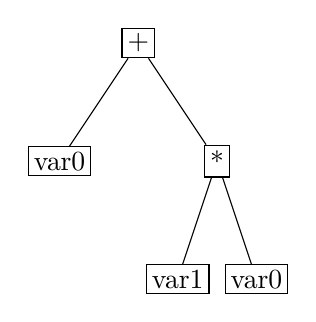
\begin{tikzpicture}
        [
        every node/.style={draw, inner sep=2pt},
        level distance=1.5cm,
        level 1/.style={sibling distance=2cm},
        level 2/.style={sibling distance=1cm}
        ]
        
        \node {+}
        child {
            node {var0}
        }
        child {
            node {*}
            child {
            node {var1}
            }
            child {
            node {var0}
            }
        };
    \end{tikzpicture}
    \caption{An example of an abstract syntax tree (AST) using deBruijn indexing. This translates to the function \texttt{f = var0 + var1 * var0}.}
    \label{fig:AST}
\end{figure}




Here, an initial DSL along with suitable syntactic constraints compile into a context-free grammar (CFG), which defines the possible structures of programs within its DSL. A CFG consists of a set of production rules that describe how to generate strings from a set of non-terminal and terminal symbols. It's "context-free" because the production rules are applied regardless of the surrounding symbols.
In DeepSynth, a prediction model is used to predict weights for a probabilistic CFG (PCFG), extending the CFG by associating probabilities with the production rules. This allows the grammar to not only generate the syntactic structure of a program but also to represent beliefs about the relative plausibility or frequency of different structures \footnote{See appendix \ref{app:cfg} for a formalization of CFGs and PCFGs.}. This is similar to DreamCoder's transition matrix which is outputted by the recognition model. The PCFG guides the search and inference process towards more likely programs. DreamCoder however, does not specifically use a PCFG. Both frameworks employ a typed $\lambda$-calculus, hence there are restrictions on program arguments, etc. (syntactical constraints). DreamCoder performs type inference during program generation. To spare computational cost, DeepSynth constructs the CFG beforehand which in turn increases the size of the CFG.

\subsubsection{\green{GFlowNet}}\label{sec:gflownet}
In the following I will give a detailed explanation of GFlowNet
\todo[inline]{should this be here or in intro? Explain why we explain this. 1. to show how the algorithm works, 2. to show how we deal with the marginalization term}

GFlowNets create a directed acyclic graph (DAG) over the state space, where vertices correspond to states or partial samples and edges denote transitions or adding a component to a partial sample, in which the edges carry a flow from source to targets \cite{bengio2023gflownet, bengio_flow_2021}.
\todo[inline]{show diagram of DAG and talk about the causality requirement! (In the methods section we explain what we do and why we do it.)}
In GFlowNets, the "flow" in the network corresponds to the process by which the network constructs a sample, which can be thought of as a path in a graph where nodes are partial samples, and edges correspond to adding a component to the partial sample.
The core training objective for a GFlowNet is to satisfy the flow matching constraint. The idea is to ensure that the flow into any state (a partially constructed sample) should match the flow out of it, given the reward associated with complete samples. The flow here refers to the expected transitions into or out of a state under the model's stochastic policy. 
Formally, a state \( s \) represents a partial object a certain stage in the generative process. A trajectory \( \tau \) is a sequence of states \( s_0, s_1, ..., s_T \) that the model traverses from an initial state \( s_0 \) to a terminal state \( s_T \), where the target structure is complete.
A trajectory \( \tau \) is formed by a sequence of actions \( a_1, a_2, ..., a_T \), where each action \( a_t \) transitions the model from state \( s_{t-1} \) to state \( s_t \). The sequence of actions is governed by a policy \( \pi \), which defines the probability of choosing a particular action given the current state.
The flow \( F(\tau) \) of a trajectory \( \tau \) is defined as the product of the probabilities of each transition along the trajectory, multiplied by the reward \( R(s_T) \) of the terminal state, normalized by a partition function \( Z \).

\begin{equation} \label{eq:flow}
    F(\tau) = \frac{R(s_T)}{Z} \prod_{t=0}^{T-1} \pi_\theta(s_{t+1} | s_{t})
\end{equation}

The partition function \( Z \) ensures that the sum of flows over all possible trajectories equals one, effectively normalizing the distribution. Since we don't know \( Z \), we can estimate it by parameterizing it as \( Z_{\theta} \).
The flow matching constraint enforces that for any given non-terminal state \( s \), the total flow into \( s \) must equal the total flow out of \( s \):

\begin{equation} \label{eq:flow_match}
    F(\tau) = F(\tau')
\end{equation}

where \( F(\tau') \) is the reverse trajectory.
We can utilize this property to create a suitable loss function to train the GFlowNet \cite{malkin_trajectory_2022}. Combining equations \ref{eq:flow} and \ref{eq:flow_match} gives us:

\begin{equation}
    \frac{R(s_T)}{Z_\theta} \prod_{t=0}^{T-1} \pi_\theta(s_{t+1} | s_{t}) = \frac{R(s_0)}{Z_\theta} \prod_{t=0}^{T-1} \beta_\theta(s_{t} | s_{t+1})
\end{equation}

Here \( \beta \) is the backward policy, predicting parent states. 
The initial state \(s_0\) has the total flow and no reward, we can rewrite it and get:

\begin{equation}
    Z_{\theta} \prod_{t=0}^{T-1} \pi_\theta(s_{t+1} | s_{t}) = R(s_T) \prod_{t=0}^{T-1} \beta_\theta(s_{t} | s_{t+1})
\end{equation}

We can now take the log on both sides:

\begin{equation}
    \log \left(Z_{\theta} \prod_{t=0}^{T-1} \pi_\theta(s_{t+1} | s_{t})\right) = \log \left(R(s_T) \prod_{t=0}^{T-1} \beta_\theta(s_{t} | s_{t+1})\right)
\end{equation}

This can be rearranged to:

\begin{equation}
    \log Z_\theta + \sum_{t=0}^{T-1} \log \pi_\theta(s_{t+1}|s_{t}) = \log R(s_T) + \sum_{t=0}^{T-1} \log \beta_\theta(s_{t}|s_{t+1})
\end{equation}

The trajectory balance loss is the squared difference:

\begin{equation}
    \mathcal{L}_{TB} = \left(\log Z_\theta + \sum_{i=0}^{T-1} \log \pi_\theta(s_{t+1}|s_{t}) - \log R(s_T) - \sum_{t=0}^{T-1} \log \beta_\theta(s_{t}|s_{t+1})\right)^2
\end{equation}

In order to mitigate the computational [cost], I am embedding all rules rather than primitives \todo[inline]{this is explained in a later section}, such that each rule is unique. Thus, every predicted node (rule) has exactly one parent, in other words, I am essentially linearising the tree. Therefore, $\beta$ will always be $1$ and can be disregarded from the equation.
Moreover, since we are solving tasks \( x \in X \), we have a conditional reward distribution $R(s_T|x)$, as well as a conditional forward policy $\pi_\theta(s_T|x)$ and partition function $Z_\theta(x)$.
This gives us the final loss:

\begin{equation}\label{form:TB}
     \mathcal{L}_{TB} = \left(\log Z_\theta(x) + \sum_{t=0}^{T} \log \pi_\theta(s_{t+1}|s_{t}, x) - \log R(s_T \vert x)\right)^2
\end{equation}     



% Formally, the computational model is as follows:
% input: tasks x in X, DSL, syntactic constraints, reward function, hyperparameters alpha, beta, epsilon, generative model, GFN

% output: trained generative model, trained recognition model, programs solving tasks X


% \subsubsection{\orange{Compositional Latent Variable Model}}
% Finetuning our fomalization, we can specify that our goal is to construct programs $z \in \mathcal{Z}$ where $z$ can be nested. We can therefore see it as a compositional latent variable model as described in \cite{hu_gflownet-em_2023}. 
% Given a set of observations \( X \), the marginal likelihood or evidence is:
% \begin{equation}\label{form:evidence}
% p(x) = \sum_z p_\theta (x|z) p_\theta(z)
% \end{equation}

% We can formalize the optimization challenge as finding the parameters \( \theta \) that maximize the data's log-likelihood:
% \begin{equation} %\label{form:bayes}
%     \mathcal{L} = \log \prod_{i=1}^{T} p(x_i) = \sum_{i=1}^{T} \log \sum_{z} p_\theta(x_i|z) p_\theta(z)
% \end{equation}

% \todo[inline]{is this correct? is the optimization challenge not over phi and theta and X?}

% The full algorithm is described in the pseudocode: \ref{alg:flowcoder}. 

\todo[inline]{We need to formalize the overall objective}

\subsubsection{\green{Expectation-Maximization}}
Hu et al. introduce a GFlowNet-EM which utilizes Expectation-Maximization in order to deal with the difficult problem of joint optimization \cite{hu_gflownet-em_2023} \footnote{See \url{https://github.com/GFNOrg/GFlowNet-EM/} for the accompanying code.}.
The core principle of Expectation-Maximization (EM) involves an iterative two-step process: the Expectation (E) step computes an expectation of the log-likelihood evaluated using the current estimate for the parameters, and the Maximization (M) step, computes parameters maximizing the expected log-likelihood found in the E-step. The GFlowNet version is slightly different and we separate the parameterization.
In the E-step the recognition model is optimized, i.e. the forward policy of the GFlowNet that is proportional to the posterior.
Here, empirical data as well as a trajectory is sampled and the trajectory balance loss is used to update the parameters of the forward policy $\pi_\phi(z|x)$, i.e. $\nabla_\phi \mathcal{L}_{TB}$.
In the M-step also empirical data and a trajectory is sampled but only the reward is used to update the parameters of the generative model $p_\theta(x \vert z) p_\theta(z)$.




\subsubsection{\green{Sleep}}
As sleep has been proven to be a crucial element of the models success, I am utilizing it too. 
\begin{description}
    \item[Replay] In Replay, I am training the forward policy on previously correctly solved task-program pairs $(x, z)$, using the trajectory to guide the model to the correct solution and optimizing on the forward logits. Here $x$ is sampled from the empirical distribution and $z$ is sampled from the forward policy $\pi_\phi$. Additionally, I apply a sleep weight $\gamma$ to strengthen the gradient. Formally:
    \begin{equation}
        \nabla_\phi\mathcal{L}_{\text{Replay}} = \mathbb{E}_{x \sim X, z \sim \pi_\phi(z|x)} \left[ - \gamma \cdot \log \pi_\phi(\tau \vert x, z) \right]
    \end{equation}
    If a correct solution has been found during the E-step, I immediately let the model train on these trajectories of correct solutions so as to consolidate these.
After the E-step I again train the model on a set (in the mathematical sense, meaning no duplicates) of all the correct solutions, so that it doesn't forget solutions to other tasks.
Replay is applied stochastically, given the hyperparameter \texttt{replay\_prob}.
    
    \item[Fantasy] During Fantasy I train the model on programs constructed during the E-step and run tasks from the empirical distribution through those programs to create correct task-program pairs $(x, z)$. Then, similarly to the methodology of Replay, I train the model on these pairs. Formally:

    \begin{equation}
        \nabla_\phi\mathcal{L}_{\text{Fantasy}} = \mathbb{E}_{x \sim X, z \sim \pi_\phi(z|x)} \left[ - \gamma \cdot \log \pi_\phi(\tau \vert x, z) \right]
    \end{equation}
    Fantasy is also applied stochastically, given the hyperparameter \texttt{fantasy\_prob}. 
    \todo[inline]{filtering out programs that produce None, constants, etc. }
    Fantasy on incorrectly proposed programs or randomly generated programs from the generative model lets the model learn which task-program pairs make sense, while fantasy on correct programs lets the model generalize solutions to different input-output pairs.
\end{description}


\subsubsection{\green{Optimization Techniques}}\label{sec:optim}
Hu et al. propose a few optimization techniques which proved to be useful \cite{hu_gflownet-em_2023}. I adapted these techniques and will describe them in the following.
\begin{description}
    \item[E-step Loss Thresholding] Rather than training the GFlowNet to a loss of zero after each M-step, we can apply a linearly decreasing moving average loss $\delta$ as a threshold to trigger the M-step using the hyperparameter $\alpha$, to save computational cost. Here I use the recursive formula:

    \begin{equation}\label{eq:threshold}
        \delta = \alpha \cdot \mathcal{L}_{TB} + (1 - \alpha) \cdot \delta
    \end{equation}
    \item[Exploration] Since we want to find many modes in the E-step and want to avoid getting stuck in local optima, several exploration techniques can be employed.
    The hyperparameter $\{\beta \vert \beta \in \mathbb{R}_{[0, 1]} \}$  can be used to exponentiate the forward policy: $ \pi_\theta(s_{t+1}|s_t)^\beta $.
    Moreover, $\epsilon$-uniform sampling can be used to the deter the model from repeating known routes by mixing the predicted logits with a uniform distribution. $\epsilon$ is chosen to be $\{\epsilon \vert \epsilon \in \mathbb{R}_{[0, 1]} \}$.
\end{description}


\begin{algorithm}[H]
    \caption{FlowCoder}
    \begin{algorithmic}[1]
    \Require Data $X$, generative model with parameters $\theta$, forward policy with parameters $\phi$, optimization and exploration hyperparameters, threshold $\alpha$
    \Repeat
        \State Sample $x \sim X$
        \State Sample $z \sim \pi_\phi(z|x)$
        \State \textbf{E-step}: gradient update on $\phi$ with $\nabla_\phi \mathcal{L}_{TB}$
        \If{$r \in (0, 1) < \texttt{replay\_prob}$}
            \State gradient update on $\phi$ with $\nabla_\phi\mathcal{L}_{\text{Replay}}$
        \EndIf
        \If{$r \in (0, 1) < \texttt{fantasy\_prob}$}
            \State gradient update on $\phi$ with $\nabla_\phi\mathcal{L}_{\text{Fantasy}}$
        \EndIf
        \If{$\mathcal{L} < \alpha$}
            \State Sample $z \sim \pi_\phi(z|x)$
            \State \textbf{M-step}: gradient update on $\theta$ with $\nabla_\theta[-\log p_\theta(x|z)p_\theta(z)]$
        \EndIf
    \Until{some convergence condition}
    \end{algorithmic}
    \label{alg:flowcoder}
    \end{algorithm}
\todo[inline]{explain algorithm, check for additional hyperparameters, etc. should the gradient update of mstep be just the reward? }






\subsection{\green{Model Architecture}}




\begin{figure*}[htbp]
    \centering
    \begin{adjustbox}{width=\textwidth}
        \begin{tikzpicture}[
            node distance=2cm, 
            auto, 
            thick,
            box/.style={
                rectangle,
                rounded corners,
                draw=black, 
                align=center,
                drop shadow,
                minimum height=1cm,
                minimum width=2cm
            },
            arrow/.style={
                ->,
                -{Stealth[length=10pt]}
            }
        ]
        
            % Nodes
            \node[box, fill=yellow!50] (task) {Task};
            \node[box, fill=yellow!70, right=3cm of task] (ioencoder) {IOEncoder};
            \node[box, fill=blue!20, below=1cm of task] (state) {State};
            \node[box, fill=blue!50, right=3cm of state] (ruleencoder) {RuleEncoder};
            
            % Positioning the Transformer node in between IOEncoder and RuleEncoder
            \coordinate (middle) at ($(ioencoder.east)!0.5!(ruleencoder.east)$);
            \node[box, fill=green!20, right=3cm of middle] (transformer) {Transformer};
            
            % Nodes for FORWARD and Z at 45 degree angles
            \node[box, fill=purple!30, above right=0.5cm and 2cm of transformer] (forward) {FORWARD};
            \node[box, fill=purple!50, below right=0.5cm and 2cm of transformer] (z) {Z};
        
            % Edges
            \draw[arrow] (task) -- (ioencoder);
            \draw[arrow] (state) -- (ruleencoder);
            \draw[arrow] (ioencoder) -- (transformer);
            \draw[arrow] (ruleencoder) -- (transformer);
            \draw[arrow] (transformer) -- (forward);
            \draw[arrow] (transformer) -- (z);
        
        \end{tikzpicture}
    \end{adjustbox}
    \caption{Insert explanation + maybe change task to an actual task; same with state; maybe also show the forward and Z output better.}
    \label{ref:model_diagram}
\end{figure*}
\todo[inline]{this looks like its one model show that the transformer output is a state representation. the GFlowNet 
 and Z takes it and produces logits.}





\begin{figure}[H]
    \centering
    % Tree 1
    \begin{subfigure}[t]{0.18\textwidth}
        \centering
        \raisebox{1.5cm}{ % Adjust vertical position
        
\begin{tikzpicture}[every node/.style={draw, circle, inner sep=2pt}]
            \node {+};
        \end{tikzpicture}
        }
        \caption{Step 1}
    \end{subfigure}
    \hspace{0.5cm} % Space between trees
    % Tree 2
    \begin{subfigure}[t]{0.18\textwidth}
        \centering
        \raisebox{0.75cm}{ % Adjust vertical position
        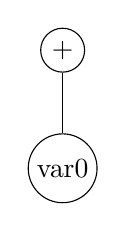
\begin{tikzpicture}[every node/.style={draw, circle, inner sep=2pt}]
            \node {+}
            child { node {var0} };
        \end{tikzpicture}
        }
        \caption{Step 2}
    \end{subfigure}
    \hspace{0.5cm} % Space between trees
    % Tree 3
    \begin{subfigure}[t]{0.18\textwidth}
        \centering
        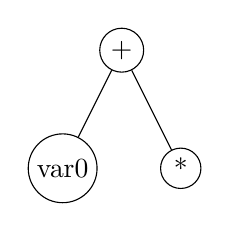
\begin{tikzpicture}[every node/.style={draw, circle, inner sep=2pt}]
            \node {+}
            child { node {var0} }
            child { node {*} };
        \end{tikzpicture}
        \caption{Step 3}
    \end{subfigure}
    \hspace{0.5cm} % Space between trees
    % Tree 4
    \begin{subfigure}[t]{0.18\textwidth}
        \centering
        \raisebox{-0.75cm}{ % Adjust vertical position
        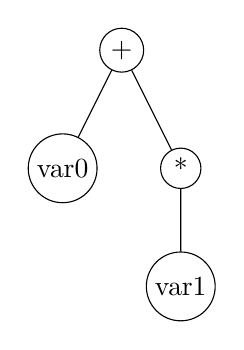
\begin{tikzpicture}[every node/.style={draw, circle, inner sep=2pt}]
            \node {+}
            child { node {var0} }
            child { node {*}
                child { node {var1} }
            };
        \end{tikzpicture}
        }
        \caption{Step 4}
    \end{subfigure}
    \hspace{0.5cm} % Space between trees
    % Tree 5
    \begin{subfigure}[t]{0.18\textwidth}
        \centering
        \raisebox{-1.5cm}{ % Adjust vertical position
        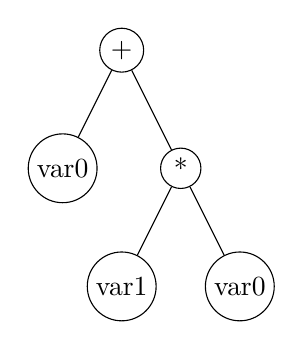
\begin{tikzpicture}[every node/.style={draw, circle, inner sep=2pt}]
            \node {+}
            child { node {var0} }
            child { node {*}
                child { node {var1} }
                child { node {var0} }
            };
        \end{tikzpicture}
        }
        \caption{Step 5}
    \end{subfigure}
    \caption{Incremental construction of the abstract syntax tree (AST) for \texttt{var0 + var1 * var0}.}
    \label{fig:AST}
\end{figure}



\begin{figure}
    \centering
    
    % Define styles for the nodes and the level distances
    \tikzset{
        every node/.style={draw, circle, inner sep=2pt},
        level distance=12mm,
        level 1/.style={sibling distance=24mm},
        level 2/.style={sibling distance=12mm},
    }
    
    % Tree at time t = 1
    \begin{subfigure}[b]{0.2\textwidth}
        \centering
        \begin{tikzpicture}
            \node {+}
                child {edge from parent[draw=none]}
                child {edge from parent[draw=none]};
        \end{tikzpicture}
        \caption*{$t = 1$}
    \end{subfigure}
    \hspace{1em} % Space between trees
    % Tree at time t = 2
    \begin{subfigure}[b]{0.2\textwidth}
        \centering
        \begin{tikzpicture}
            \node {+}
                child {node {pow}}
                child {edge from parent[draw=none]};
        \end{tikzpicture}
        \caption*{$t = 2$}
    \end{subfigure}
    \hspace{1em} % Space between trees
    % Tree at time t = 3
    \begin{subfigure}[b]{0.2\textwidth}
        \centering
        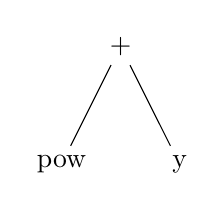
\begin{tikzpicture}
            \node {+}
                child {node {pow}}
                child {node {y}};
        \end{tikzpicture}
        \caption*{$t = 3$}
    \end{subfigure}
    \hspace{1em} % Space between trees
    % Tree at time t = 4
    \begin{subfigure}[b]{0.2\textwidth}
        \centering
        \begin{tikzpicture}
            \node {+}
                child {node {pow}
                    child {node {y}}
                    child {edge from parent[draw=none]}
                }
                child {edge from parent[draw=none]};
        \end{tikzpicture}
        \caption*{$t = 4$}
    \end{subfigure}
    
    % Tree at time t = 5
    \begin{subfigure}[b]{0.2\textwidth}
        \centering
        \begin{tikzpicture}
            \node {+}
                child {node {pow}
                    child {node {y}}
                    child {node {x}}
                }
                child {edge from parent[draw=none]};
        \end{tikzpicture}
        \caption*{$t = 5$}
    \end{subfigure}
    
    \caption{Creation of a five node tree using the grow initialization method with a maximum depth of 2, using terminal set $T$ and function set $F$ defined earlier, ($t = $ time).}
    \label{fig:growth_trees}
    \end{figure}
    


% All modules are written using PyTorch \cite{NEURIPS2019_9015}.
See table \ref{table:params} for the exact parameterization of the model.


\subsubsection{\green{Generative Model}}
To embed programs effectively within a neural network, it is essential to represent them in a format that is compatible with the neural network's architecture. Abstract syntax trees, which are inherently 2-dimensional and include information of parent, children and sibling nodes, should be translated into a neural network format while ensuring the preservation of this valuable structural information.
Various concepts have emerged, including using Graph Neural Networks (GNNs), e.g. see \cite{allamanis2017learning, velickovic_clrs_2022, Bieber_Sutton_Larochelle_Tarlow_2020, ibarz2022generalist}. Others proposed special Tree-Transformers which are able to encode ASTs, see e.g. \cite{peng_rethinking_2022, Wang_Lee_Chen_2019}.
He et al. find that standard Transformers achieve similar results to Transformers where tree position information is explicitly encoded \cite{he_trees_2021}. This is presumably because of the positional encoding, which is a way of adding fixed sinusoidal functions with different frequencies and phases to the embeddings of tokens in a sequence, enabling the neural network to discern the position of each tokens through these distinctive patterns; and more importantly, because of the fundamental component of the Transformer, which is the self-attention mechanism, formalized as \cite{Vaswani_Shazeer_Parmar_Uszkoreit_Jones_Gomez_Kaiser_Polosukhin_2017}:
\begin{equation}
    \text{Attention}(Q, K, V) = \text{softmax}(\frac{QK^T}{\sqrt{d_k}})V
\end{equation}

This mechanism, through the query (Q), key (K), and value (V) matrices, allows the model to dynamically assign importance to different parts of the input sequence. The scaling factor $\sqrt{d_k}$ normalizes the dot product, aiding in stabilizing gradients during training. Moreover, the Transformer employs Multi-Head Attention, enabling the model to concurrently process information from different representation subspaces, enhancing its capability to capture diverse features. 
Therefore, I decided to use the standard Transformer architecture, which takes a 1-dimensional sequence as an input, meaning the AST has to be linearized. 

Rather than embedding the primitives of the DSL to construct ASTs, I embed the already preprocessed rules of the context-free grammar, created in conjunction with the syntactic constraints, thus essentially predicting edges rather than nodes. The array of CFG rules has to be converted back to AST format for evaluation, which can be easily done within the DeepSynth framework.
In a plausible model of cognition, we don't possess an explicit representation of the CFG but rather infer it.
However, in the case of DeepSynth, it generates a more extensive CFG instead of conducting type inference, which is the approach employed in DreamCoder. Consequently, I must perform a lookup to identify the syntactically permitted rules, thereby filtering out those that do not conform to the syntax. Naturally, in principle, I could allow the model to generate syntactically incorrect programs and assign them a reward of 0 during evaluation, but to expedite the learning process, I refrain from doing so.

\begin{description}
    \item[The RuleEncoder] begins by collecting rules, which are pairs of non-terminals and corresponding program actions, from the CFG and adds special tokens such as 'PAD' (padding), 'START' (sequence start), and 'STOP' (sequence end). Each rule is passed through a PyTorch embedding layer.
    During the forward pass, batches of state sequences (each state sequence, or trajectory $\tau$, representing a series of CFG rules) are processed. To ensure uniformity across different sequences within a batch, padding is applied.
    \item[The IOEncoder] is tasked with encoding input-output (IO) pairs into continuous vector representations.
    Each input-output pair is tokenized using a predefined lexicon (a list of symbols representing the possible range of inputs and outputs), which includes special tokens such as 'PAD' (padding), 'IN' (input start), and 'OUT' (output start). This tokenization is critical for distinguishing between different parts of the input-output pairs.
    The tokenized input-output pairs are concatenated into a single sequence, with the 'IN' and 'OUT' tokens demarcating the transition from input to output. Padding is then applied to ensure that all sequences have the same length, aligning them to the maximum allowed size determined by \texttt{n\_examples\_max} (the maximum number of input examples that can be processed) and \texttt{size\_max} (the maximum size of elements in a list). These parameters have been adapted from DeepSynth. The padded sequences are passed through a PyTorch embedding layer. This embedding is crucial for capturing the semantic relationships between different tokens.
    \item[The Transformer] initializes with the IOEncoder and the RuleEncoder. Positional Encoding is applied to the output of both encoders. This step is vital as it adds information about the sequence order to the model, allowing the Transformer to interpret the sequence data effectively.
    The Transformer employs two types of masks: padding masks for IO sequences and square subsequent masks for state sequences. The padding mask ensures that the model does not process padding tokens, while the square subsequent mask prevents positions from attending to subsequent positions, maintaining the autoregressive property in the generation process.
\end{description}

\subsubsection{\green{Forward Policy}}
At each step, the forward policy takes the Transformer output as an encoded state and predicts log probabilities over the CFG rules, after which I apply softmax to get a distribution between 0 and 1 and sample the next action. 
The forward policy is implemented as a Multi-Layer Perceptron (MLP) and predicts forward logits from the Transformer's output, guiding the generative process.

\subsubsection{\green{Partition Function}}
The partition function $Z_\theta$ serves as a normalizing factor, ensuring that the probabilities generated by the model are well-calibrated and interpretable. It is implemented as a MLP layered on top of the Transformer output.

\subsubsection{\green{Sampling Programs}}
In the process of constructing an Abstract Syntax Tree, there exists flexibility in the order of expansion. Nodes can be expanded in a depth-first, breadth-first, etc. manner, or for instance, one can adopt a bottom-up approach, wherein terminal nodes are predicted initially and subsequently connected in a progressive manner. This approach offers the advantage of enabling the evaluation of partial expressions, which, in turn, can serve to inform the model and enhance computational efficiency, albeit at the expense of increased memory requirements. Alternatively, we may consider employing a model akin to the forward policy, predicting the subsequent node (or edge) to be expanded.
However, I chose to sample the actions for the tree construction in a depth-first manner. I did this for two reasons. 
First, for simplicity, to not overcomplicate the model, and second so that the AST when linearized, always has the same order, potentially giving the Transformer a useful inductive bias.

Specifically, the state of each program in the batch is initialized with a 'START' token, representing the initial state of the program generation process. A frontier, implemented as a queue, is initialized for each program to manage the sequence of non-terminals that need to be expanded. This method has been adapted from DeepSynth to fit with the FlowCoder framework and mechanisms. 
The core of the method is a loop that continues until all frontiers are empty, indicating that all programs in the batch have been fully generated. Within this loop, the model computes logits and partition functions.
As discussed in section \ref{sec:optim}, the sampling method includes an exploration mechanism, where with a probability $\epsilon$, uniform sampling is used instead of the model's logits. This exploration is crucial for introducing variability and avoiding local optima in the generation process. Additionally, tempering is applied to logits using a factor $\beta$, modulating the sharpness of the probability distribution used for sampling.
For each program in the batch, the method iteratively samples a rule based on the current non-terminal and updates the program's state and cumulative logits. This process involves creating a mask to block invalid actions, applying the mask to logits, and sampling an action (rule) based on the masked logits.
Each sampled rule is decomposed into a non-terminal and program component, updating the program's current state and expanding the frontier with the rule's arguments.
Once all frontiers are empty, the final programs are reconstructed from their compressed representations, using methods provided by DeepSynth.

\todo[inline]{Refer to program construction diagram}
\todo[inline]{detailed algorithm of replay and fantasy}

\subsubsection{\green{Reward}}
In order to train the model, we need to operationalize a reward function. Various approaches exist for this purpose, the simplest being a binary reward, as employed in DreamCoder. Does the output of the program match the actual output or not? A binary reward however, is not very informative. A reward that provides a gradient is much more useful. Bengio et al. propose an Energy-Based Model (EBM), wherein the model learns to associate favorable outcomes with low energy states and unfavorable outcomes with high energy states \cite{bengio2023gflownet}. Depending on the domain, this may be useful but in my experiments, working in the list editing domain, however, I found that it introduced unnecessary complexity to the model. Instead, I am using the Levenshtein edit distance, using the \texttt{Levenshtein} package \footnote{\url{https://github.com/maxbachmann/Levenshtein}}, which is a measure of the similarity between two strings. Specifically, it quantifies the minimum number of single-character edits (i.e., insertions, deletions, or substitutions) required to transform one string into another. See appendix \ref{app:levenshtein} for an in depth formalization of the metric.
Since the Levenshtein distance returns a discrete value, I normalize it over the maximum length of the sequences, and since there may be more than one example per task, I average it over all examples. Moreover, I apply a maximum reward parameter, to scale a correct solution up and give the model a stronger gradient. In my experiments I used a maximum reward of 10.















\subsection{\green{Design}}
In the following section I will elaborate on the exact training and test methods I used, including hyperparameters.
The tasks I am using are input-output relations in the list editing domain, originally from DreamCoder, see Table \ref{tab:task_ex} for examples. These were filtered given the syntactic constraints (e.g. type, lexicon, etc.) and provided by DeepSynth. 
In their paper, Fijalkow et al. discuss that some of the tasks are impossible solve given the DSL, so I additionally filtered those out. In my experiments I end up with 95 tasks. Tasks can be of a similar variety (e.g. \texttt{add-k with k=1} and \texttt{add-k with k=2} belong to the same group). There are 25 such task groups in total. Each task can have between 1 and 15 examples. A task is considered solved if a program solves all examples of the task \footnote{All tasks can be found in my GitHub repository.}.
The DSL is essentially a dictionary of primitive types and semantics in a typed $\lambda$-calculus, including functions like \texttt{index}, \texttt{car}, \texttt{append} as well as numerical functions like \texttt{+}, \texttt{*}, \texttt{mod}, \texttt{is-prime}, etc., all written in Python (see appendix \ref{app:dsl}).
Table \ref{tab:synconst} describes the syntactical constraints used in the experiment, which were mostly adapted from DeepSynth and DreamCoder.

\begin{table}[H]
    \centering
    \begin{tabularx}{\textwidth}{|l|l|X|}
        \hline
        \textbf{Parameter} & \textbf{Value} & \textbf{Description} \\\hline
        \texttt{type} & \texttt{list(int) $\rightarrow$ list(int)} & The input as well as the output should be a list of integers, so the CFG should reflect that, filtering rules that do not conform to that criterion. \\\hline
        \texttt{lexicon} &  $[-30, 30] \in \mathbb{Z}$ & The lexicon is a uniform distribution of integers and in the range from -30 to 30 \\\hline
        \texttt{maximum argument number} & 1 & This is the maximum number of arguments a function could have. \\\hline
        \texttt{size max} & 10 & The maximum number of values in a list \\\hline 
        \texttt{max number of examples} & 15 & The maximum number of examples per task \\\hline 
    \end{tabularx}
    \caption{Syntactical Constraints}
    \label{tab:synconst}
\end{table}

All experiments were trained in random order with a batch size of 4 where each task in the batch is the same. This was done to avoid a credit assignment problem while increasing efficiency. Since the forward logits are summed up and averaged over for all trajectories, training the model at multiple task at once might have confused which trajectory was rewarding. However, batching, especially when training on a GPU has computational benefits.
Furthermore, each task is trained for 5 epochs with 2.000 E-steps and 2.000 M-steps in each epoch. The moving average threshold (see equation (\ref{eq:threshold})) $\delta$ was initialized with 150 and linearly decreases using the hyperparameter $\alpha$ set to 0.3. The exploration parameters $\beta$ and $\epsilon$ were set to $0.7$ and $0.3$, respectively. The sleep weight $\gamma$ was set to 10 on all experiments. 
The learning rates for the generative model as well as for the forward policy were set to $0.0001$. During inference I ran the model for $100$ steps. Since the batch size is 4, this creates 400 programs per task. A table of all hyperparameters can be found in Table \ref{tab:hyperparams} of appendix \ref{app:hyperparams}. The experiments were run on a single NVIDIA Tesla T4 GPU. Throughout the five epochs, each consisting of 2.000 E- and M-steps with a batch size of four, the model generated approximately 80.000 programs per task.

\begin{table}[H]
    \centering
    \begin{tabular}{|p{5cm}|c|c|}
        \hline
        \textbf{Task} & \textbf{Input} & \textbf{Output} \\\hline
        \texttt{remove gt 2} & \texttt{[1,2,7,5,1]} & \texttt{[1,2,1]} \\\hline
        \texttt{caesar-cipher-k-modulo-n with k=5 and n=4} & \texttt{[2, 2, 0, 1, 2, 3, 3]} & \texttt{[3, 3, 1, 2, 3, 0, 0]} \\\hline
        \texttt{prepend-index-k with k=3} & \texttt{[15, 12, 9, 14, 7, 9]} & \texttt{[9, 15, 12, 9, 14, 7, 9]} \\\hline
        \texttt{add-k with k=4} & \texttt{[16, 10, 7, 12, 13, 3]} & \texttt{[20, 14, 11, 16, 17, 7]} \\\hline
        \texttt{append-k with k=2} & \texttt{[1, 5, 15]} & \texttt{[1, 5, 15, 2]} \\\hline
    \end{tabular}
    \caption{Task Examples}
    \label{tab:task_ex}
\end{table}



\begin{table}[H]
    \centering
    \begin{tabular}{|p{5cm}|c|}
        \hline
        \textbf{Task} & \textbf{Program} \\\hline
        \texttt{remove gt 2} & \texttt{(filter (gt? 3) var0)} \\\hline
        \texttt{caesar-cipher-k-modulo-n with k=5 and n=4} & \texttt{(map (mod 4) (map (+ 5) var0))} \\\hline
        \texttt{prepend-index-k with k=3} & \texttt{(cons (index 2 var0) var0)} \\\hline
        \texttt{add-k with k=4} & \texttt{(map (+ 4) var0)} \\\hline
        \texttt{append-k with k=2} & \texttt{(append 2 var0)} \\\hline
    \end{tabular}
    \caption{Examples of tasks and programs solving the tasks.}
    \label{tab:task_programs}
\end{table}
